\PassOptionsToPackage{sols}{handout}
\documentclass[main]{subfiles}
\setcounterrefbeforedot{chapter}{m-ws6-7}
\setcounterrefafterdot{section}{m-ws6-7}
\addtocounter{section}{-1}
\usepackage{solutions}

\begin{document}

\ifSubfilesClassLoaded{%
  \chaptermark{\chaptersix}
}{}

\section{More Density Problems} \label{ws6-7}

\begin{problemonly}
    \begin{framed}

\textbf{Key Idea}:

\begin{itemize}[topsep=0pt,partopsep=0pt,parsep=8pt,itemsep=0pt]


\item You should develop more flexibility with density problems and be
  able to apply our strategy from last time to 3-dimensional regions.

\end{itemize}
\end{framed}
\end{problemonly}

\begin{enumerate}
\item 
  Farmer Joe and Farmer Bob have identical circular corn fields of
  radius 100 meters.  However, they have different ideas about how to
  water their fields.
  \begin{enumerate}
  \item Farmer Joe decides to install a single high-powered sprinkler
    right in the center of his corn field.  Corn grows better near the
    sprinkler, so the yield density of corn in Farmer Joe's field is given
    by $\displaystyle j(x) = \frac{10000}{1 + x^2}$ stalks of corn per
    square meter, where $x$ is distance from the sprinkler.  We'd like to
    find out how much corn Farmer Joe's field yields.

    \begin{enumerate}
    \item
      \begin{problem}[1.5in]
        Show in a sketch the meaning of $x$ in Farmer Joe's field.  Then
        show in a sketch how you would \textbf{slice} Farmer Joe's field.
      \end{problem}    

      \begin{solution}
        Here is a plot showing the yield density in the field (red
        represents the highest density and purple represents the lowest).
        Since $x$ represents distance from the center, we can actually
        draw the $x$-axis in \emph{any} direction, as long as it's 0 at
        the center and 100 at the edge:
        \begin{center}
          \begin{tikzpicture}
            \begin{axis}[x=0.007in, y=0.007in, xmin=0, xmax=115, ymin=-100,
              ymax=100, axis on top=true, clip=false, hide y axis,
              xtick={100}, xlabel=$x$, tick label style={fill=none}] 
              \draw (0, 0) node{
\includegraphics[width=1.4in]{images/circular-cornfields-rings-density-crop.pdf}};
            \end{axis}
          \end{tikzpicture}
        \end{center}
        As always, we want to slice the region so that the density in each
        slice is almost constant.  In this case, we can accomplish that by
        slicing into concentric rings.  (All of the points within a single
        ring are approximately the same distance from the sprinkler, so
        they have approximately the same yield density.)  This means that
        we're slicing the interval $[0, 100]$ into $n$ pieces of equal
        width, and we'll label the endpoints $x_0 = 0, \ldots, x_n =
        100$. 
        \begin{center}
          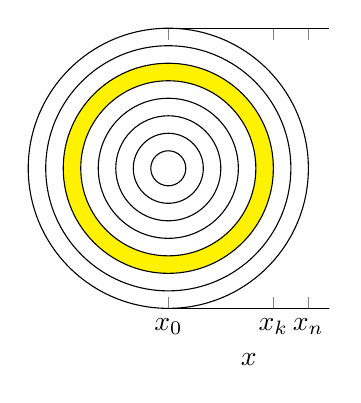
\begin{tikzpicture}
            \begin{axis}[x=0.007in, y=0.007in, xmin=0, xmax=115,
              ymin=-100, ymax=100, axis on top=true, clip=false, hide y
              axis, xtick={0.1, 75, 100}, xticklabels={$x_0$, $x_k$, $x_n$},
              xlabel=$x$, tick label style={fill=none}]              
              \draw[fill=yellow, draw=none] (0, 0) circle(75); %
              \draw[fill=white, draw=none] (0, 0) circle (62.5); %
              \pgfplotsforeachungrouped \x in {12.5, 25, ..., 100.1}
              {
                \edef\temp{
                  \noexpand\draw (0, 0) circle(\x);
                }
                \temp
              }              
            \end{axis}
          \end{tikzpicture}
        \end{center}
      \end{solution}

    \item
      \begin{problem}[\stretch{1}]
        How would you \textbf{approximate} the corn yield of the $k$-th
        slice?
      \end{problem}    

      \begin{solution}
        As usual,
        \[ \text{corn yield of $k$-th slice} \approx (\text{corn yield
          density in $k$-th slice})(\text{area of $k$-th slice}).\] The
        corn yield density in the $k$-th slice is approximately
        $\rho(x_k)$.  Since the $k$-th slice is a ring with outer radius
        $x_k$ and thickness $\Delta x$, its area is approximately $2 \pi
        x_k \Delta x$.  Therefore, the corn yield of the $k$-th slice is
        approximately $\boxed{\rho(x_k) \cdot 2 \pi x_k \Delta x}$.
      \end{solution}

    \item
      \begin{problem}[\vfill]
        Write a general Riemann \textbf{sum} that approximates the total
        yield of Farmer Joe's corn field.
      \end{problem}

      \begin{solution}
        Summing our answer from {\enumiiprefix {{{\#1}}}{(a)}ii} over
        all slices, the yield of Farmer Joe's corn field is approximately
        \fbox{$\displaystyle \sum_{k=1}^n \rho(x_k) \cdot 2 \pi x_k \Delta
          x$}.
      \end{solution}

    \item

      \note{I may not have them actually evaluate this integral,
        but I will see if they
        can think of a useful substitution.}

      \begin{problem}[\vfill]
        By \textbf{taking an appropriate limit}, find a definite integral
        that gives the exact yield of Farmer Joe's field. 
      \end{problem}

      \begin{solution}
        Taking the limit as $n \to \infty$ of the general Riemann sum we
        found gives the integral
        \begin{align*}
          \boxed{\int_0^{100} \rho(x) \cdot 2 \pi x \,dx} &= 20000 \pi \int_0^{100}
          \frac{x}{1 + x^2}\,dx \\
          \intertext{Let's substitute $u = 1 + x^2$; then, $du = 2x\,dx$,
            so $\frac{du}{2} = x\,dx$.  As $x$ goes from $0$ to ${100}$, $u =
            1 + x^2$ goes from $1 + 0^2 = 1$ to $1 + {100}^2 = 10001$:}
          &= 20000 \pi \int_1^{10001} \frac{1}{u} \cdot \frac{du}{2} \\
          &= 10000 \pi \int_1^{10001} \frac{1}{u}\,du \\
          &= 10000 \pi \ln u \Big|_1^{10001} \\
          &= \boxed{10000 \pi \ln 10001 \text{ stalks of corn}}
        \end{align*}
      \end{solution}

    \end{enumerate}

\pspace{\newpage}

  \item

    \note{Again, if there is time, I'll ask them how we might evaluate
      this integral, without working out all of the details; this one is
      trickier since we need to split it up and use geometry on one
      piece.}

    \begin{problem}[\vfill]
      Farmer Bob decides to install a 200 meter long straight irrigation
      pipe in his corn field.  The pipe runs right down the center of the
      plot, and the corn density in Farmer Bob's plot varies with distance
      to the pipe.  If the density is given by $b(x) = 200 - x$ corn
      stalks per square meter, where $x$ is distance to the pipe, write a
      definite integral that gives the number of corn stalks in Farmer
      Bob's field. 
    \end{problem}

    \begin{solution} 
      As usual, we want to slice the region so that the density in each
      slice is approximately constant.  In this case, density varies with
      distance to the pipe, so we'll need to slice parallel to the pipe.
      Let's visualize the pipe running vertically through the center of
      the field:
      \begin{center}
        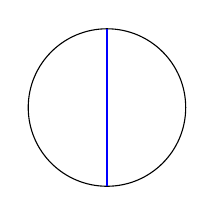
\begin{tikzpicture}
          \draw (0, 0) circle (1);
          \draw[blue, thick] (0, -1) -- (0, 1);
        \end{tikzpicture}
      \end{center}
      By symmetry, the left and right halves of the field have the same
      amount of corn, so we can just focus on the right half of the field.
      In fact, symmetry tells us that, if we cut the field both
      horizontally and vertically through the center, each quarter has the
      same amount of corn, so let's just focus on the top right quadrant
      of the field.  Remembering that $x$ measures the distance from the
      pipe, here is a picture of the quarter field with the $x$-axis:
      \begin{center}
        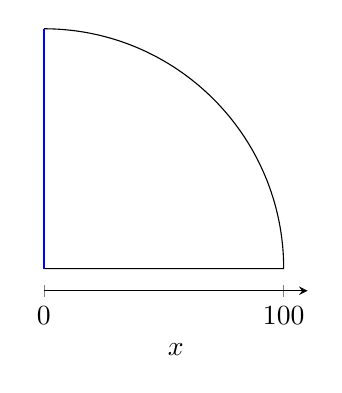
\begin{tikzpicture}
          \begin{axis}[xmin=0, xmax=110, ymin=0, ymax=100, x=0.012in,
            y=0.012in, hide y axis, axis x line=bottom, clip=false,
            xlabel=$x$, xtick={0, 100}]  
            \begin{scope}[yshift=8pt]
              \draw (0, 0) -- (100, 0) arc[radius=100, start angle=0, end
              angle=90]; %
              \draw[blue, thick] (0, 0) -- (0, 100);
            \end{scope}
          \end{axis}
        \end{tikzpicture}
      \end{center}
      Slicing parallel to the pipe means slicing the interval $[0, 100]$;
      as usual, we'll slice into $n$ pieces of equal thickness $\Delta x$
      and label the values where we sliced as $x_0 = 0, x_1, \ldots, x_n =
      100$.  Let's focus on the $k$-th slice:
      \begin{center}
        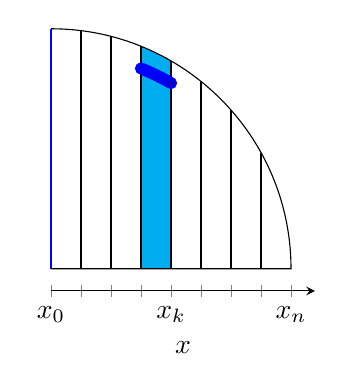
\begin{tikzpicture}
          \begin{axis}[xmin=0, xmax=22, ymin=0, ymax=20, x=0.06in,
            y=0.06in, hide y axis, axis x line=bottom, clip=false,
            xlabel=$x$, xtick={0, 2.5, 5, ..., 20.1},
            xticklabels={$x_0$,,,,$x_k$,,,,$x_n$}] 
            \begin{scope}[yshift=8pt]
            \addplot+[domain=7.5:10, fill=cyan, draw=none,yshift=-8pt]
              {sqrt(20^2-x^2)} -- (10, 0) -- (7.5, 0);
              \draw (0, 0) -- (20, 0) arc[radius=20, start angle=0, end
              angle=90]; %
              \draw[blue, thick] (0, 0) -- (0, 20);
              \pgfplotsforeachungrouped \x in {2.5, 5, ..., 19.9}
              {
                \edef\temp{
                  \noexpand\draw (\x, 0) -- (\x, {sqrt(20^2-\x^2)});
                }
                \temp
              }              
            \end{scope}
          \end{axis}
        \end{tikzpicture}
      \end{center}
      The yield of the $k$-th slice is approximately $(\text{yield density
        in $k$-th slice})(\text{area of $k$-th slice})$.  The yield
      density in the $k$-th slice is approximately $\rho(x_k)$.  To
      approximate the area of the $k$-th slice, we can approximate the
      slice as a rectangle of width $\Delta x$.  However, we still need to
      express its height in terms of $x_k$.  The key is to use the shape
      of the field: it's part of a circle, so we need to use the radius.
      If we draw in the radius (shown in red) below, then we can express
      the height $h_k$ in terms of $x_k$:
      \begin{center}
        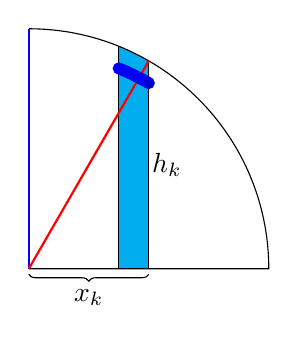
\begin{tikzpicture}
          \begin{axis}[xmin=0, xmax=22, ymin=0, ymax=20, x=0.06in,
            y=0.06in, hide y axis, axis x line=bottom, clip=false,
            xlabel=$x$, xtick=\empty, hide x axis] 
            \begin{scope}[yshift=8pt]
              \addplot+[domain=7.5:10, fill=cyan, draw=none,yshift=-8pt]
              {sqrt(20^2-\x^2)} -- (10, 0) -- (7.5, 0); %
              \draw (7.5, 0) -- (7.5, {sqrt(20^2-7.5^2)}); %
              \draw (10, 0) -- node[right, inner sep=1pt] {$h_k$} (10,
              {sqrt(20^2-10^2)}); %
              \draw (0, 0) -- (20, 0) arc[radius=20, start angle=0, end
              angle=90]; %
              \draw[blue, thick] (0, 0) -- (0, 20); %
              \draw[decorate, decoration={brace, mirror}, yshift=-2pt] (0,
              0) -- node[yshift=-2pt, below] {$x_k$} (10, 0); %
              \draw[red, thick] (0, 0) -- (10, {sqrt(20^2-10^2)}); %
            \end{scope}
          \end{axis}
        \end{tikzpicture}
      \end{center}
      We now see a right triangle in the picture: the hypotenuse is the
      radius of the field, which is 100; the two legs have length $x_k$
      and $h_k$.  Therefore, by the Pythagorean Theorem, $x_k^2 + h_k^2 =
      100^2$, so $h_k = \sqrt{100^2 - x_k^2}$.  So, we can approximate the
      area of this slice as $h_k \Delta x = \sqrt{100^2 - x_k^2}$.
      Therefore,
      \[ \text{yield of $k$-th slice} \approx \rho(x_k) \cdot \sqrt{100^2
        - x_k^2} \Delta x.\]
      Summing over all slices and taking the limit as the number of slices
      $\to \infty$, the yield of one quarter of Farmer Bob's plot is
      $\displaystyle \int_0^{100} \rho(x) \cdot \sqrt{100^2 - x^2}\,dx$.
      Therefore, the yield of Farmer Bob's plot is
      \begin{align*}
        \boxed{4 \int_0^{100} \rho(x) \cdot \sqrt{100^2 - x^2}\,dx} &= 4
        \int_0^{100} (200 - x) \sqrt{100^2 - x^2}\,dx \\
        \intertext{To evaluate this integral, let's expand the integrand:}
        &= 4 \int_0^{100} \left( 200 \sqrt{100^2 - x^2} - x \sqrt{100^2 -
            x^2} \right) dx \\
        &= 800 \int_0^{100} \sqrt{100^2 - x^2}\,dx - 4 \int_0^{100} x
        \sqrt{100^2 - x^2}\,dx \\
        \intertext{We don't know an antiderivative of $\sqrt{100^2 -
            x^2}$, but you should recognize that its graph is the top half
          of the circle of radius 100 centered at the origin.  Therefore,
          we can visualize $\displaystyle \int_0^{100} \sqrt{100^2 -
            x^2}\,dx$ as the area of a quarter circle of radius 100, so
          this integral is equal to $\frac{1}{4} \cdot \pi \cdot 100^2$.
          For the second integral, let's substitute $u = 100^2 - x^2$;
          then, $du = -2x\,dx$, so $-\frac{du}{2} = x\,dx$.}
        &= 800 \cdot \frac{1}{4} \cdot \pi \cdot 100^2 - 4 \int_{100^2}^0
        \sqrt{u} \left( - \frac{du}{2} \right) \\
        &= 2,000,000 \pi + 2 \int_{100^2}^0 u^{1/2}\,du \\
        &= 2,000,000 \pi + \left( \left. 2 \cdot \frac{2}{3}
            u^{3/2} 
          \right|_{100^2}^0 \right) \\
        &= 2,000,000 \pi - \frac{4}{3} \cdot 100^3 \\
        &= \boxed{2,000,000 \pi - \frac{4,000,000}{3}}
      \end{align*}
    \end{solution}

  \end{enumerate}

\pspace{\newpage}

\item 
 % From Robin's Spring 2007 in-class worksheet

  \begin{problem}[\vfill]
    A cone with height $8$ inches and radius $6$ inches is filled with
    flavored slush. When the cup is held upright with the pointed end
    resting on a table, the density of flavoring syrup in the cup varies
    with height above the table.  Suppose $\rho(x) = \frac{1}{x + 1}$
    gives the number of ounces of syrup per cubic inch, where $x$ is the
    distance from the table top.  Write an integral giving the total
    amount of syrup in the cup.
  \end{problem}

  \begin{solution}
    First, let's make sure we understand the meaning of $x$ in this
    problem.  Since $x$ represents distance from the table top, $x = 0$ at
    the tip of the cone and $x = 8$ at the top.

    As always, the key in density problems is to slice so that the density
    within each slice is approximately constant.  This allows us to
    reasonably approximate the amount (of syrup, in this case) in each
    slice by multiplying the density within the slice by the volume of the
    slice.  Since the density varies with height, we will slice the cone
    parallel to the table.  This amounts to slicing the interval $[0, 8]$
    (on the $x$-axis).  As usual, we'll focus on the $k$-th slice (the
    whole slice is shown to the left):
    \begin{center}
      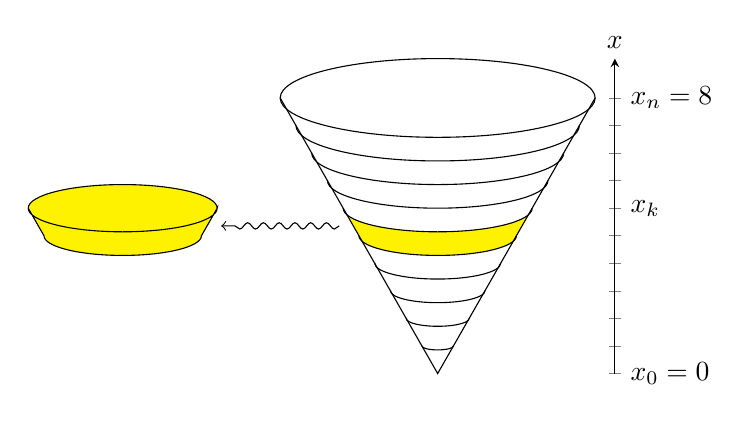
\begin{tikzpicture}[x=0.5cm, y=0.5cm]

        \begin{axis}[xmin=-4, xmax=4.5, ymin=0, ymax=8, clip=false, hide
          x axis, axis y line=right, x=0.5cm, y=0.5cm, ytick={0, 0.7, ...,
            7.01}, yticklabels={$x_0 = 0$,,,,,,$x_k$,,,,$x_n = 8$}]
            \coordinate (right) at (4, 7);
            \coordinate (left) at (-4, 7);
            \coordinate (tip) at (0, 0);
          \draw[fill=yellow, draw=none] (2, 3.5) arc[x radius=2,
          y radius=0.5, start angle=0, end angle=-180] -- (-2.4, 4.2)
          arc[x radius=2.4, y radius=0.6, start angle=180, end
          angle=360] -- cycle; %
          \draw (right) arc[x radius=4, y radius=1, start angle=0, end
          angle=180]; %
          \draw (right) -- (tip) -- (left); %
          \draw (4.5, 8) node[above] {$x$}; %
          \pgfplotsforeachungrouped \y in {0, 0.7, ..., 7.01} {
            \pgfmathsetmacro{\x}{4/7*\y} %
            \edef\temp{%
              \noexpand\draw (\x, \y) arc[x radius=\x, y radius={\x/4},
              start angle=0, end angle=-180];
            }              
            \temp
          }
          \draw [->,decorate, decoration={snake,amplitude=.4mm,segment
            length=2mm,post length=1mm}]  (-2.5, 3.75) -- (-5.5, 3.75);
          \begin{scope}[xshift=-4cm]
            \draw[fill=yellow, draw=none] (2, 3.5) arc[x radius=2, y
            radius=0.5, start angle=0, end angle=-180] -- (-2.4, 4.2)
            arc[x radius=2.4, y radius=0.6, start angle=180, end
            angle=360] -- cycle; %
            \draw[fill=yellow, draw=none] (2.4, 4.2) arc[x radius=2.4, y
            radius=0.6, start angle=0, end angle=360]; %
            \draw (2.4, 4.2) arc[x radius=2.4, y radius=0.6, start
            angle=0, end angle=360] -- (2, 3.5) arc[x radius=2, y
            radius=0.5, start angle=0, end angle=-180] -- (-2.4, 4.2); %
          \end{scope}
        \end{axis}
      \end{tikzpicture}
    \end{center}
    The $k$-th slice looks approximately like a disk of thickness $\Delta
    x$, so we can approximate its volume as $\pi (\text{radius})^2 \Delta
    x$.  However, we must express the radius in terms of $x_k$; we can do
    this using similar triangles.  Let's call the radius we want $r_k$: 
    \begin{center}
      \begin{tikzpicture}[x=0.5cm, y=0.5cm]
        

        \begin{axis}[xmin=-4, xmax=4.5, ymin=0, ymax=8, clip=false, hide
          x axis, axis y line=right, x=0.5cm, y=0.5cm, ytick={0, 0.7, ...,
            7.01}, yticklabels={$x_0 = 0$,,,,,,$x_k$,,,,$x_n = 8$}]
            \coordinate (right) at (4, 7);
        \coordinate (left) at (-4, 7);
        \coordinate (tip) at (0, 0);
          \draw[fill=yellow, draw=none] (2, 3.5) arc[x radius=2,
          y radius=0.5, start angle=0, end angle=-180] -- (-2.4, 4.2)
          arc[x radius=2.4, y radius=0.6, start angle=180, end
          angle=360] -- cycle; %
          \draw (right) arc[x radius=4, y radius=1, start angle=0, end
          angle=360]; %
          \draw (right) -- (tip) -- (left); %
          \draw (4.5, 8) node[above] {$x$}; %
          \draw[dashed] (2.4, 4.2) arc[x radius=2.4, y radius=0.6, start
          angle=0, end angle=180]; % 
          \pgfplotsforeachungrouped \y in {3.5, 4.2} {
            \pgfmathsetmacro{\x}{4/7*\y} %
            \edef\temp{%
              \noexpand\draw (\x, \y) arc[x radius=\x, y radius={\x/4},
              start angle=0, end angle=-180];
            }              
            \temp
          }
          \draw[red] (tip) -- ($0.5*(right)+0.5*(left)$) -- (right) --
          cycle;
          \draw[red] (0, 4.2) -- node[above, inner sep=0.5pt] {$r_k$}
          (2.4, 4.2); 
        \end{axis}
      \end{tikzpicture}
    \end{center}
    The larger triangle in the picture has height 8 and width 6; the
    smaller triangle has height $x_k$ and width $r_k$.  So, $\frac{6}{8} =
    \frac{r_k}{x_k}$, which means $r_k = \frac{6}{8} x_k = \frac{3}{4}
    x_k$.  Therefore,
    \begin{align*}
      \text{volume of $k$-th slice} &\approx \pi \left( \frac{3}{4} x_k
      \right)^2 \Delta x \\
      & = \frac{9 \pi}{16} x_k^2 \Delta x \text{ cubic inches} \\
      \text{density of syrup in $k$-th slice} & \approx \rho(x_k)
      \text{ ounces per cubic inch}\\
      \text{amount of syrup in $k$-th slice} & \approx \rho(x_k) \cdot 
      \frac{9 \pi}{16} x_k^2 \Delta x \\
      & = \frac{9 \pi}{16} x_k^2 \rho(x_k)
      \Delta x \text{ ounces}
    \end{align*}
    Summing over all slices, the amount of syrup in the cup is
    approximately $\displaystyle \sum_{k=1}^n \frac{9 \pi}{16} x_k^2
    \rho(x_k) \Delta x$.  Taking the limit as $n \to \infty$, the amount
    of syrup in the cup is exactly \fbox{$\displaystyle \int_0^8 \frac{9
        \pi}{16} x^2 \rho(x)\,dx$}.
  \end{solution}

\end{enumerate}

\end{document}
